% Kapitel 6

\chapter{Adding Depth Information to 2D U-Nets for CT Segmentation} % Main chapter title
\label{chap:semi-3d}

In the previous two chapters, we discussed two specific methods of model-driven preprocessing and their extensions. In this chapter, we will introduce a preprocessing technique designed to incorporate depth information into 2D images, aiming to bridge the gap between 2D and 3D image segmentation. CT scans, being 3D images, are often segmented with 3D neural networks. However, directly segmenting 3D scans poses two key challenges:

Firstly, 3D scans are naturally very large, as instead of processing one e.g. $256 \times 256$ slice, the network now needs to process a $256 \times 256 \times 256$ volume. This dramatically increases memory requirements and restricts the maximum batch size. In extreme cases where processing an entire scan is infeasible, the data is either partitioned into smaller patches \cite{zhu3DCoarsetoFineFramework2018}, downsampled with focused re-segmentation on regions of interest \cite{isenseeNnUNetSelfconfiguringMethod2021}, or segmented using semi-3D networks \cite{wenConvolutionalNeuralNetworks2020}.

Secondly, the scarcity of large 3D datasets exacerbates the risk of overfitting, as we have established that using large images necessitates the use of high-capacity models. Segmenting individual slices, on the other hand, can act as a form of regularization, creating multiple samples from a single subject and allowing for the use of smaller networks.

Therefore, there is a need for methods that can effectively integrate depth information into 2D segmentation networks, maintaining the technical benefits of a 2D network while enhancing them with depth perception.

One potential solution to incorporate depth information into 2D segmentation networks is to condition the network's output on the slice depth by adding the slice depth coordinate as an additional input feature. This would give the network more information about the expected segmentation shape as a function of slice depth both globally and individually for that slice. However, integrating such scalar information into a fully convolutional network like U-Net is not straightforward.

This problem has been solved in the field of image generation, where the condition is added as a separate input channel. For an image \(I \in \mathbb{R}^{W \times H \times C}\) and a condition vector \(x\), the image is augmented to include \(\lvert x \rvert\) additional channels. Each new channel \(c(i) \in \mathbb{R}^{W \times H}\) is constructed so that every pixel \(c(i)_{xy}\) equals \(x(i)\) for all \(x, y\) coordinates \cite{mirzaConditionalGenerativeAdversarial2014}. This approach is illustrated in \figref{fig:conditioned-image}.

\begin{figure}[t!]
    \centering
    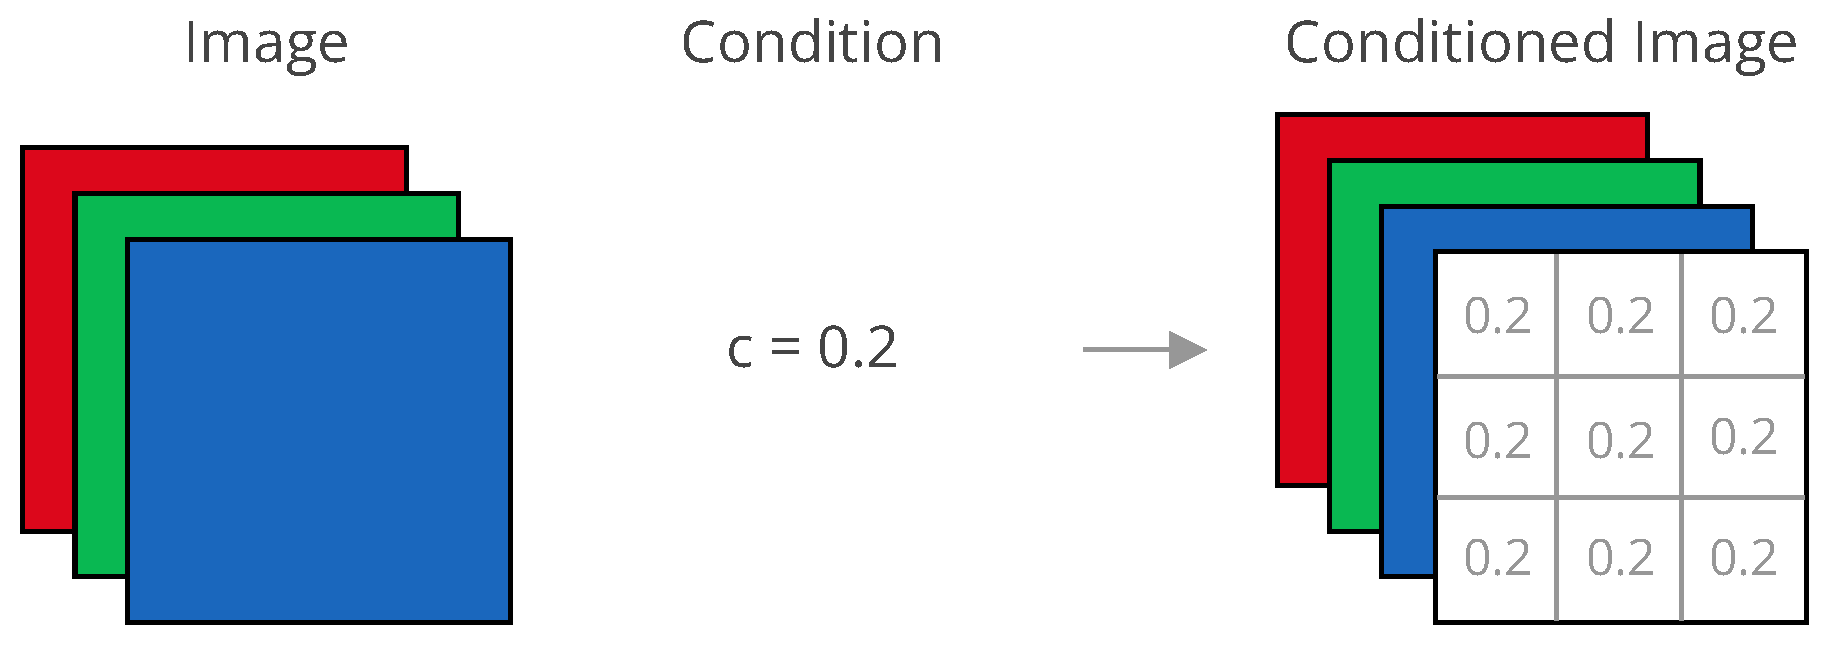
\includegraphics[width=0.65\columnwidth]{images/6/conditioned-image}
    \caption{An illustration of conditioning an image by adding a channel to the image where each pixel is equal to the condition value.}
    \label{fig:conditioned-image}
\end{figure}

Drawing inspiration from this, we propose a new and simple way of incorporating 3D information into 2D fully-convolutional neural networks for medical image segmentation. Consider a 3D scan comprising \(D\) slices:
\begin{equation}
	I = \{I_d(x, y)\; \vert\;  I_d(x,y) \in R^{W \times H}, d \in [1..D]\}.
\end{equation}
For every slice \(I_d\), we create a depth information channel \(C_d(x, y) = d / D\) for all \(x, y\), i.e. each pixel is equal to the normalized z-coordinate of that slice. The network's input for each slice becomes $I'_{d} = [I_d, C_d]$ where the first channel is $I_d$ and the second channel contains the depth information.

This method enables 2D networks to utilize depth cues without significant modifications to their architecture or an increase in parameter count, maintaining compatibility with transfer learning from 2D datasets. Throughout the rest of this chapter, we evaluate this technique on the specific task of epicardial adipose tissue (EAT) segmentation.

\section{Epicardial Adipose Tissue Segmentation}

Epicardial adipose tissue (EAT) is a type of adipose tissue located within the pericardium, a protective layer around the heart. EAT lies between the myocardium (the heart muscle) and the fibrous outer layer of the pericardium. Due to EAT's proximity to the myocardium, it is believed to be a metabolically active organ that has a direct impact on various cardiovascular diseases.

For instance, EAT has been shown to play a direct role in coronary atherosclerosis and cardiomyopathy \cite{Sacks2007, Marwan2013}. EAT thickness has been shown to correlate with metabolic syndrome \cite{Chenn2009} and coronary artery disease independently of obesity \cite{Iacobellis2011}. It relates in general with the progression of coronary artery calcification \cite{Gorter2008}. Additionally, the volume and density of EAT have been linked to major adverse cardiac events in asymptomatic subjects \cite{Goeller2018}. Additionally, EAT plays a role in insulin resistance, is an accurate therapeutic target, and impacts heart morphology and adiposity \cite{Iacobellis2009-2}.

EAT's active role in cardiovascular diseases makes measuring its volume and thickness an important diagnostic tool. Currently, EAT is most often quantified by measuring EAT thickness using echocardiography. This estimation of the volume from the thickness at a single point can introduce inaccuracies and inter-observer variability. Using 3D medical imaging technologies such as CT results in more accurate measurements, however, the availability of CT machines as well as the procedure's cost and duration make it impractical for common clinical use. Another downside of using CT to measure EAT is the time required to manually measure EAT volume, which can take up to an hour per patient \cite{Militello2019} and is prone to inter-observer variability of around 10\% \cite{Marwan2013} of the measured volume. Fully or semi-automatic methods of EAT segmentation and quantification from CT images could reduce time requirements and the cost of EAT quantification.

Segmenting EAT is a challenging image-processing task. Its uneven distribution around the heart, peculiar shape, and its similarity to other adipose tissues nearby complicate the process. Segmenting EAT relies on delineating the pericardium, which is less than 2 mm thin and can often be hard to delineate on CT images due to partial volume effects.

\section{Related Work}

Incorporating depth information into 2D segmentation networks often involves training on preselected regions of interest, where multi-channel images are constructed from sequential slices of a 3D volume \cite{wenConvolutionalNeuralNetworks2020}. These multi-slice images serve as input for conventional 2D networks. Our approach diverges by directly supplying the z-coordinate as an additional input channel. Similar strategies are employed in U-Net-based architectures in image generation, such as Imagen \cite{sahariaPhotorealisticTexttoImageDiffusion2022}. We suggest that a similar method of incorporating supplementary information could improve the data efficiency of image segmentation tasks.

There are several semi-automatic and fully automatic methods for EAT segmentation proposed in the existing literature. One of the first methods of EAT segmentation was proposed by \citet{Coppini2010}. They use a semi-automatic approach where an expert places control points on the pericardium which are used to segment the pericardium using thresholding and geodesic active contours. An improved semi-automatic segmentation method is presented by \citet{Militello2019}. Their method requires expert input to define the VoI on a few slices of the scan, and the rest of the VoI is then interpolated, saving time while still offering manual-level segmentation accuracy.

\citet{Ding2014} propose a method similar to \citet{Coppini2010} but instead of relying on manual initialization, they initialize the pericardium contour using an atlas-based method achieving fully automatic segmentation. \citet{Rodrigues2016} propose a fully automatic machine-learning-based method. Their method consists of extracting hand-selected salient features from the CT slices, which are then segmented by a learned random forest classifier.

\citet{Commandeur2018} proposed one of the first EAT segmentation methods to use deep learning. They use a multi-task approach consisting of two convolutional neural networks to classify whether a slice contains the heart and segment the pericardium as well as EAT. More recent works propose deep learning methods based on variations of the U-Net architecture. \citet{Li2019} use a U-Net with a pyramid pooling structure, while \citet{he2020} use a 3D-based U-Net with an added attention mechanism. \citet{Zhang2020} use two stacked U-Net-based networks. The first network segments a pericardium region, which is then refined using morphological operators. This region is used as a mask for the input into the other U-Net, which segments the EAT region. While similar, our approach differs from this work in several ways. We only use one U-Net-based neural network, significantly reducing the number of parameters. Additionally, we modify the input data to allow the network to utilize slice-depth information during training and inference.

\section{Dataset Description}\label{data}

We use a dataset of CT scans of 20 patients from Rio de Janeiro obtained and released publicly by \citet{Rodrigues2016}. The original ground truth was obtained via manual segmentation of 878 total slices by a physician and a computer scientist. The slices were also registered, scaled, and cropped to a similar anatomical region, as well as thresholded to the adipose tissue range of $[-200, -30]$ HU. Of the 20 patients, 10 are male and 10 are female. The mean age of the patients is 55.4. Each scan has an average of 42.95 slices with a slice thickness of 3 mm. The CT scans were obtained with two different scanners, 9 patients were scanned by a Phillips scanner, while the other 11 were scanned by a Siemens scanner.

The original labels contain three classes: pericardium, EAT, and paracardial adipose tissues. Using these labels as a reference, we manually labeled a closed pericardium region on each slice. During labeling, we follow the pericardium line where available and mark the pericardium region as the border separating the two adipose tissues when a label is not visible. We then create a separate set of EAT labels by multiplying the input images, thresholded to the range of adipose tissue, with the pericardium label. I.e. we define EAT as all adipose tissue masked by the pericardium label. A comparison of the original label and our re-labeled images is shown in \figref{fig:dataset-relabel}.

\begin{figure}[t!]
    \centering
    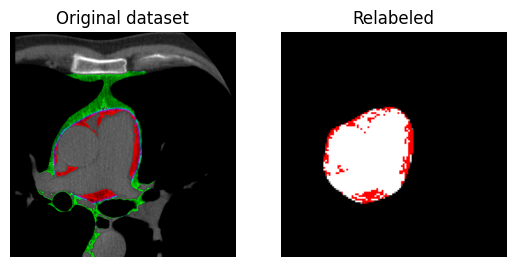
\includegraphics[width=0.65\columnwidth]{images/6/relabel}
    \caption{An example of the original image label and our relabeled image. The EAT label is shown in red, while the pericardium label is shown in white. \cite{bencevicEpicardialAdiposeTissue2021}}
    \label{fig:dataset-relabel}
\end{figure}

\section{Methodology}\label{method}

We achieve segmentation of the pericardium using a deep neural network architecture based on U-Net \cite{ronneberger2015unet}. The input to the model is a 2-channel $128 \times 128$ image. The first channel is a single slice of a patient's CT scan. The second channel, as described earlier in the chapter, represents the slice depth of that slice. The pericardium region varies highly by slice depth. Therefore, we utilize depth information by first normalizing the slice depth of each input slice to a value between 0 and 1. We then create a $128 \times 128$ image where each pixel has the value of the slice depth. This image is used as the second channel of the neural network input. This allows the network to utilize additional depth information without changing the underlying architecture. Example input images are shown in \figref{fig:input-images}.

\begin{figure}[b]
\center

\includegraphics[width=\columnwidth]{images/6/inputs.png}
\caption{A sample of the inputs to the neural network from a single patient, sorted by slice depth. The first channel (CT adipose tissue) is shown in full white, while the second channel (the slice depth) is shown from black (highest z-axis) to green (lowest z-axis). \cite{bencevicEpicardialAdiposeTissue2021}}
\label{fig:input-images}
\end{figure}

We use a loss function which is a modified version of the Dice coefficient:
  \begin{equation}
    \textit{DSC}_{loss} = 1 - \frac {2 \lvert X\cap Y \rvert + \lambda}{\lvert X \rvert + \lvert Y \rvert + \lambda},
    \label{eq:loss}
  \end{equation}
where $X$ and $Y$ are the input and predicted images, respectively, and $\lambda$ is a smoothing parameter set to 1 in our experiments.

\subsection{Data Preprocessing}

We apply several data preprocessing steps on the original dataset to achieve better segmentation results. First, the images are all normalized and zero-centered by subtracting the global mean intensity of all pixels of the training dataset (0.1). The images are then scaled down from $512 \times 512$ to $128 \times 128$ pixels. We also removed a total of 112 slices from the original dataset that did not include EAT labels, either because of labeling errors in the original dataset or because the slices were outside the heart region.

Furthermore, we utilize heavy data augmentation to increase model generalizability. In real-world distributions, anatomical structures can differ drastically from one person to the next. To simulate these differences, we add a random chance of augmenting each input image during the training phase. Each input image has a 50\% chance for a horizontal flip, and a 30\% chance of a random combination of affine image transformations, including (1) a translation of max. 6.25\% of the image's width, (2) a scaling of max. 10\% of the image's scale, and (3) a rotation of a max. 45 degrees. Additionally, each input image has a 20\% chance of a non-linear mesh deform. Examples of augmented images are shown in \figref{fig:augment}.

\begin{figure}[b!]
\center
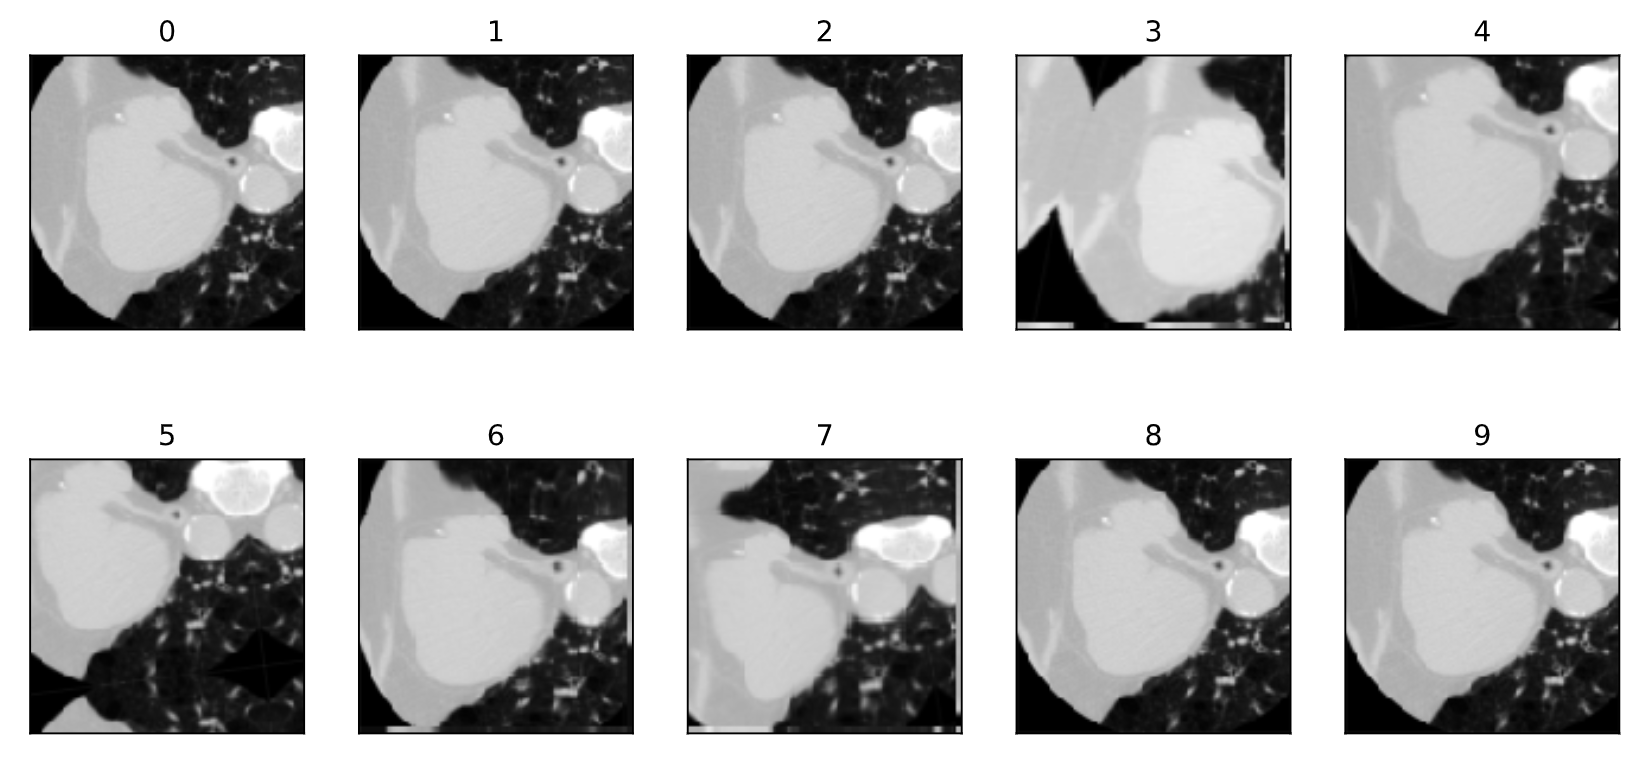
\includegraphics[width=\textwidth]{images/6/augmentation.png}
\caption{Different random augmentation examples of the same input image. \cite{bencevicEpicardialAdiposeTissue2021}}
\label{fig:augment}
\end{figure}

\subsection{Model Training}

The neural network is implemented and trained using PyTorch 1.7.1 on an NVIDIA GeForce RTX 3080 GPU. The networks were trained for 200 epochs, with a checkpoint mechanism after each epoch. We select the model with the best validation loss during training. In our experiments, the model converged around epoch 100 after 5 minutes. The training was done using the Adam optimizer with a learning rate of 0.001. The used batch size was 8. We used a manual random seed value of 42 for all experiments. We use 2-fold per-patient cross-validation for all experiments. Each model was trained on the slices of 10 patients and validated on the remaining 10 patients.

\section{Experiments and Results}\label{experiment}

The results in this section are evaluated on the two cross-validation folds and averaged across folds. Segmentation quality is evaluated using the Dice Similarity Coefficient (DSC) and the Jaccard Index. We analyze the model's quantification quality with a Bland-Altman analysis \cite{MARTINBLAND1986307} as well as with the Pearson correlation coefficient. To calculate the Pearson correlation and to perform the Bland-Altman analysis, we threshold all segmented pericardium regions to obtain the EAT segmentation results and calculate the number of pixels labeled as EAT on each image. We also calculate the number of EAT pixels on the ground truth images. The pixel counts are used as a proxy for volume measurement, as the EAT volume of a patient is proportional to the number of segmented EAT pixels in the patient's CT scan.

\subsection{Results}

Our method's mean DSC and correlation results are presented in Table \ref{tab:results}. 

\begin{table}[b!]
\renewcommand{\arraystretch}{1.4}
\caption{Mean results of the cross-validation. The Corr. value is the Pearson correlation between the total number of EAT pixels for each slice of the validation dataset ($p<0.0001$).}
\centering
\begin{tabularx}{\textwidth}{Xccccc} 
 Target & DSC & Jaccard & Prec. & Rec. & Corr. \\
 \hline
 Pericardium & 0.9264 & 0.8819 & 0.9319 & 0.9345 & - \\ 
 EAT & 0.8646 & 0.7807 & 0.8787 & 0.8690 & 0.8864 \\
\end{tabularx}
\label{tab:results}
\end{table}

The network provides better results for pericardium segmentation than EAT segmentation, which is expected given the pericardium's smoother shape. The DSC for EAT indicates that our method performs slightly worse inter-observer variability, but still achieves good segmentation in a fraction of the time needed for manual segmentation. The precision and recall have similar values both for EAT and the pericardium, showing a good potential for future use to measure EAT volume. Examples of predictions from our model are presented in \figref{fig:examples}.

\begin{figure}[b!]
    \centering
    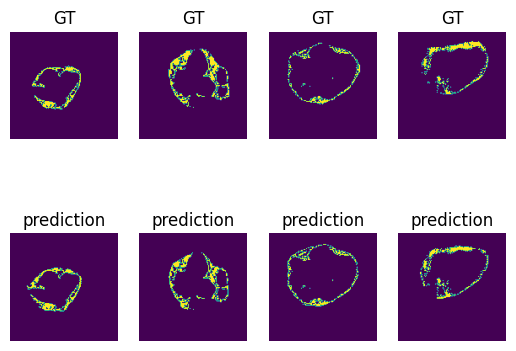
\includegraphics[width=0.7\columnwidth]{images/6/examples.png}
    \caption{Examples of EAT predictions compared to the ground truth images. \cite{bencevicEpicardialAdiposeTissue2021}}
    \label{fig:examples}
\end{figure}

The Bland-Altman analysis of our method is presented in \figref{fig:corr}. The analysis shows a high level of agreement between our method and ground-truth annotations. The plot also shows a small positive bias from our method. Additionally, the plot does not show a strong proportional bias. However, while most measurements fall within the 95\% confidence interval, there are outliers. The most likely reason for these errors is the noisy nature of the ground truth labels especially towards the edges of the heart region.

\begin{figure}[t!]
    \centering
    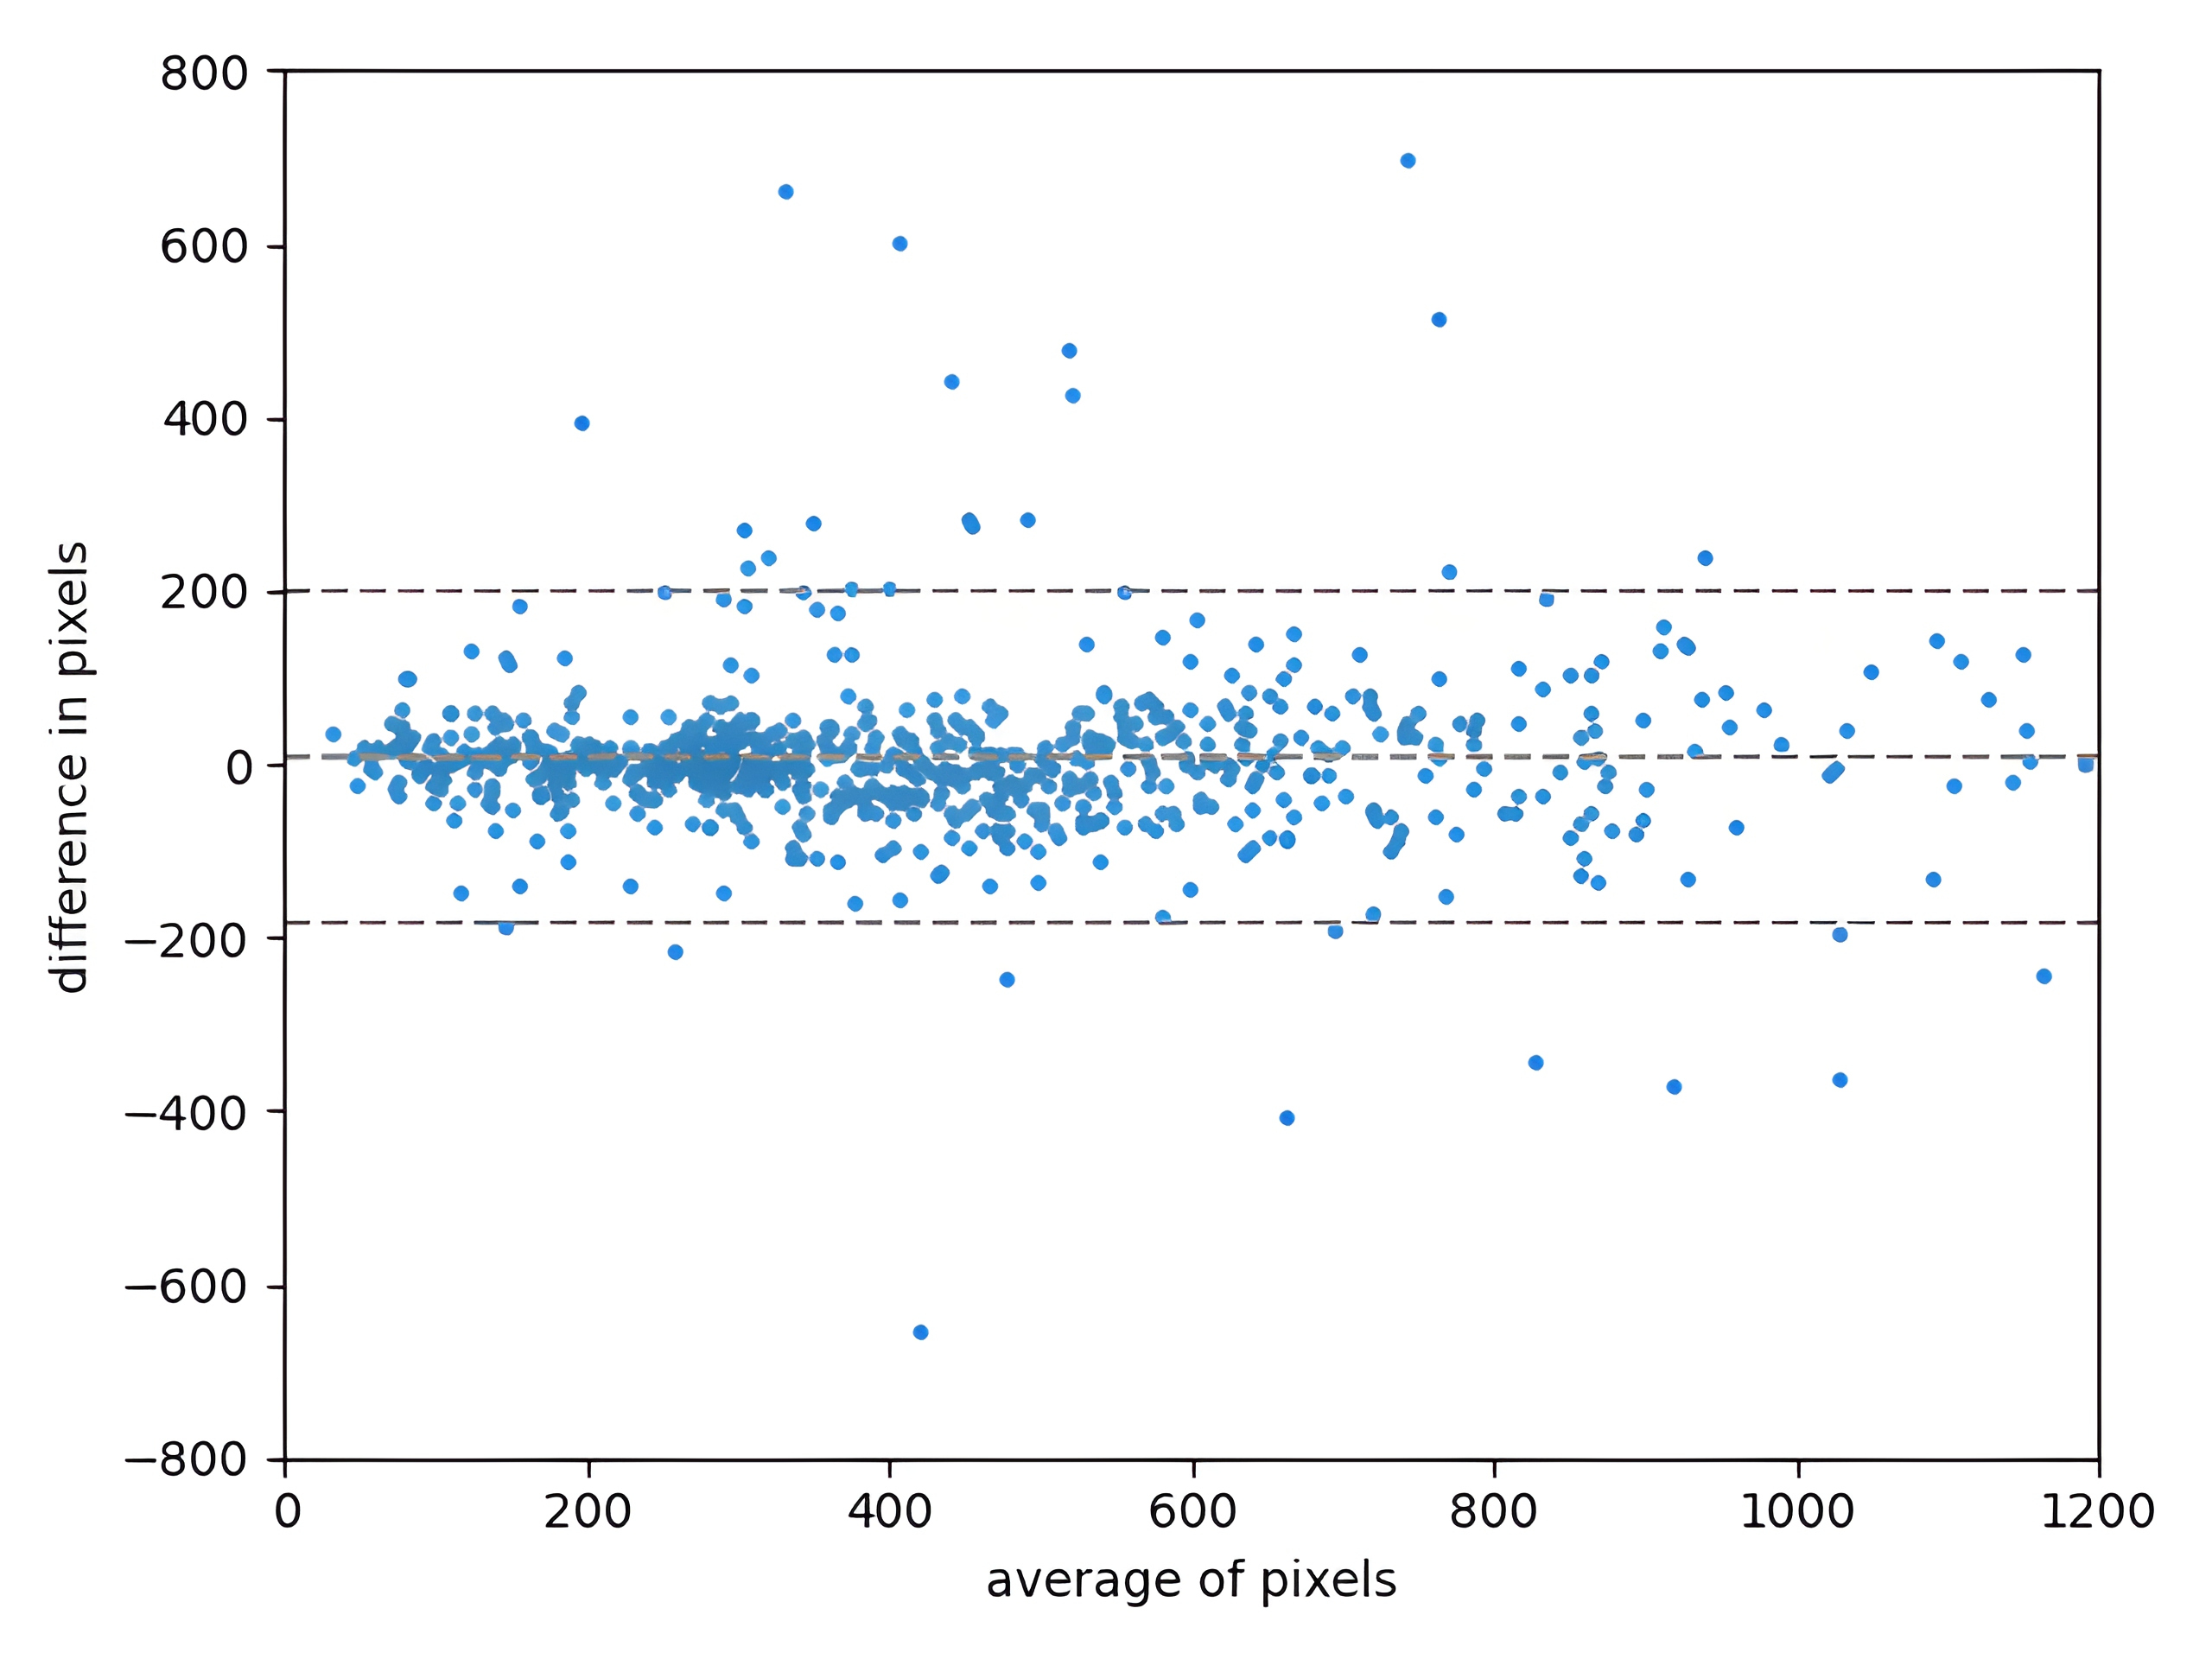
\includegraphics[width=0.75\columnwidth]{images/6/blaltman.jpg}
    \caption{The Bland-Altman analysis of the number of pixels predicted as EAT on each slice of the test dataset for each fold. The dashed lines indicate a 95\% confidence interval. \cite{bencevicEpicardialAdiposeTissue2021}}
    \label{fig:corr}
\end{figure}

Additionally, we compare our results to using a U-Net to directly segment the pericardium, as well as with other state-of-the-art approaches This comparison is presented in Table \ref{tab:comparison}.

\begin{table}[t!]
\renewcommand{\arraystretch}{1.4}
\caption{A comparison of our approach with other deep-learning-based approaches for EAT segmentation.}
\centering
\begin{tabularx}{\textwidth}{Xccccc} 
 Method & DSC & Jaccard & Prec. & Rec. & Params \\
 \hline
 U-Net for EAT & 0.75 & 0.58 & 0.72 & 0.69 & 5.8 M \\ 
 Zhang et al. \cite{Zhang2020} & \textbf{0.91} & \textbf{0.84} & - & - & 11.6 M \\
 He et al. \cite{he2020} & 0.85 & - & 0.86 & 0.89 & 6.4 M \\
 Our method & 0.86 & 0.78 & 0.89 & 0.87 & 5.8 M \\
\end{tabularx}
\label{tab:comparison}
\end{table}

\section{Conclusion}\label{conclusion}

Our approach achieved a mean Dice Similarity Coefficient (DSC) of 0.8574 and a correlation coefficient of 0.8864. Although these figures fall short of the state-of-the-art, it's important to note that our dataset underwent relabeling to minimize noise and errors, making direct comparisons to results from the original dataset challenging. In addition, our method uses a more direct neural network with fewer preprocessing steps and fewer parameters than existing deep-learning methods (\cite{Commandeur2018, Li2019, he2020}), leading to lower inference times.  We demonstrate the effectiveness of segmenting the pericardium region as a proxy for directly segmenting epicardial adipose tissue (EAT), leveraging the simpler task of learning the smooth contour of the pericardium compared to the more complex, irregular distribution of EAT. Furthermore, we explore incorporating depth information into an encoder-decoder neural network without resorting to 3D volume patch training. By adding slice depth as an extra channel we have improved segmentation performance without changing the underlying architecture and while maintaining the ability to use transfer learning from 2D datasets. The method presented in this chapter was published in \cite{bencevicEpicardialAdiposeTissue2021}.
